%%%%%%%%%%%%%%%%%%%%%%%%%%%%%%%%%%%%%%%%%
% FRI Data Science_report LaTeX Template
% Version 1.0 (28/1/2020)
% 
% Jure Demšar (jure.demsar@fri.uni-lj.si)
%
% Based on MicromouseSymp article template by:
% Mathias Legrand (legrand.mathias@gmail.com) 
% With extensive modifications by:
% Antonio Valente (antonio.luis.valente@gmail.com)
%
% License:
% CC BY-NC-SA 3.0 (http://creativecommons.org/licenses/by-nc-sa/3.0/)
%
%%%%%%%%%%%%%%%%%%%%%%%%%%%%%%%%%%%%%%%%%


%----------------------------------------------------------------------------------------
%	PACKAGES AND OTHER DOCUMENT CONFIGURATIONS
%----------------------------------------------------------------------------------------
\documentclass[fleqn,moreauthors,10pt]{ds_report}
\usepackage[english]{babel}
\usepackage{listings}
\usepackage{subcaption}
\usepackage{adjustbox}
\usepackage{verbatim}
\usepackage{tabularx}
\usepackage{multirow}
\graphicspath{{fig/}}




%----------------------------------------------------------------------------------------
%	ARTICLE INFORMATION
%----------------------------------------------------------------------------------------

% Header
\JournalInfo{FRI Natural language processing course 2024}

% Interim or final report
\Archive{Project report} 
%\Archive{Final report} 

% Article title
\PaperTitle{LLM Prompt Strategies for Commonsense-Reasoning Tasks} 

% Authors (student competitors) and their info
\Authors{Matic Pristavnik Vrešnjak, Mitja Kocjančič, and Songeun Hong}

% Advisors
\affiliation{\textit{Advisors: Slavko Žitnik}}

% Keywords
\Keywords{Large Language Models (LLMs), Prompt Strategies, Comparative Analysis}
\newcommand{\keywordname}{Keywords}


%----------------------------------------------------------------------------------------
%	ABSTRACT
%----------------------------------------------------------------------------------------
\Abstract{
The surge in the popularity of Large Language Models (LLMs) such as chatGPT, PaLM, and Gemini has led to their widespread adoption in both personal and commercial domains. Many of these cutting-edge models rely on the transformer architecture. With the increasing use of LLMs, there is a growing need to devise prompts that facilitate the generation of relevant and informative responses, particularly for tasks necessitating commonsense reasoning. Such tasks draw upon everyday knowledge for resolution. Consequently, various prompt strategies have emerged to enhance model performance on such tasks. In response to the expanding array of prompt strategies, this paper offers a comprehensive comparison of each approach, aiming to shed light on their effectiveness and applicability in enhancing LLM performance.
}

%----------------------------------------------------------------------------------------

\begin{document}

% Makes all text pages the same height
\flushbottom 

% Print the title and abstract box
\maketitle 

% Removes page numbering from the first page
\thispagestyle{empty} 

%----------------------------------------------------------------------------------------
%	ARTICLE CONTENTS
%----------------------------------------------------------------------------------------

\section*{Introduction}

    %Matic: Mockup of the introduction. You can change any part that you don't like about this text :).
    %Matic: I need some time to think about the finish up of the introduction.
    %Matic: I will take a one last look at this but I think I sholud be fine after today
    Recent years have seen a rise in the popularity of Large language models (LLMs). LLMs such as chatGPT, PaLM, Gemini, and others have already been adopted for personal and commercial use. Many of the current state-of-the-art models are based on the transformer architecture\cite{DBLP:journals/corr/VaswaniSPUJGKP17}. Because of the wide adoption of LLMs, it has become more important to provide prompts that encourage the model to generate relevant and informative responses to tasks that require commonsense reasoning. Tasks that require commonsense reasoning are those that require everyday knowledge to solve. This has led to the development of several strategies for providing prompts that allow models to perform better on such tasks. Due to the growing number of prompt strategies, we present a comprehensive comparison of each strategy.


    %Matic: I am debating if we should split this part into two sections. One for the introduction and one for related work
    %Sienna: I think it would be good to split two sections.
    %Matic: Ok

    \section*{Related work}
    %Matic: If you two find any methods that look interesting describe them here.
    %Matic: Added a small bit about Chains of thought in DSPy since the assistant mentioned this when I was talking to him. Sorry for the late add, I remembered at the last moment.
    One strategy for providing prompts is Chain of thought (CoT)\newline\cite{wei2023chainofthought}. The core idea of CoT is that we give the model a demonstration of how to come to the solution or ask it for a step-by-step response. CoT has been proven to improve the performance of LLMs on commonsense reasoning and mathematical datasets. One limitation mentioned in the original CoT paper was that CoT only benefits large models like chatGPT and not smaller models. Frameworks like DSPy\cite{khattab2023dspy} have also integrated functionality that enables the implementation of custom Chains of thought. Strategies with similar approaches are In-context Learning\cite{luo2024incontext} and Plan-and-Solve Techniques\cite{wang2023planandsolve}.
    
    Another example of prompt strategies is Promptbreeder\cite{fernando2023promptbreeder}. In contrast to methods like CoT, which are based on hand-crafted prompts, Promptbreeder can generate optimized prompts. Promptbreeder relies on LLM and genetic algorithms to mutate a set of prompts, which are then given to the LLM. Strategies that use generated prompts have been shown to perform better than the prompt strategies that are based on hand-crafted prompts.

    The aforementioned strategies are more complex and require additional text to be added to the instruction. Simpler strategies are more oriented towards creating prompts that are clear and precise\cite{chen2023unleashing}. This includes forming unambiguous and specific prompts, allowing the model to give better and more detailed answers. Research has also shown that models can provide better answers when given emotional prompts\cite{li2023large}.
    
    %Matic: Sorry about the model references. They have so many authors. If it looks too weird I can remove them. I fix this by using et al -> Good! It looks more clear.
    Previously mentioned strategies have been tested on various LLMs. LLMs that are most commonly used for testing are chatGPT\cite{openai2024gpt4}, PaLM\cite{chowdhery2022palm}, Gemini\cite{geminiteam2023gemini} and other models. Most researchers prefer to use models with a large number of parameters because larger LLMs benefit more from prompt engineering. This has led to very little research being done on smaller models.
    
    %Matic I added some related work for datasets to related work 
    %Sienna: I checked references 7, 8, 9. Thank you for adding these. 
    Because of the growing number of prompting strategies, many datasets have been used to measure their performance. Examples of such datasets are the Winograd Schema Challenge\cite{levesque2012winograd}, Textbook Question Answering\cite{Kembhavi2017AreYS},  SocialIQA\cite{sap2019socialiqa}, and many other datasets. Many of the mentioned datasets were made to challenge LLM on commonsense sense reasoning tasks.

%Matic: I need to fix the positining of the figures or at least make sure that the don't cause empty space to form
%Mitja: Empty space decreased a little bit above equasions, but figures look fine to me, unless you are bothered by Figure 7 which is on its own page
\section*{Methodology}

Various prompting strategies were tested on models obtained from the Hugging Face library. The largest models for text generation on Hugging Face have around 150 billion parameters. Unfortunately, we couldn't use these models because of the limited data storage on the HPC cluster.

\textbf{Mistral}, developed by Mistral AI, despite its relatively small size (only 7B parameters),it has demonstrated comparable performance to models like LLama3 and GPT-3.5. One notable drawback of this model is its tendency to suffer from hallucinations, which can cause it to veer off-topic.

\textbf{ROUGE}, a set of metrics commonly used in natural language processing, evaluates performance in text summarization and translation. The metrics offered by ROUGE include:
\begin{itemize}
\item Precision, measures the accuracy of positive predictions made by a model, calculated as the ratio of true positive predictions to the total number of positive predictions. A perfect score is 1, and the worst is 0.

\setlength{\abovedisplayskip}{1pt}
\begin{equation}
	\label{eqn:Precision}
	Precision = \frac{\text{True Positives}}{\text{True Positives} + \text{False Positives}}
\end{equation}


\item \textbf{Recall}, also known as sensitivity or true positive rate, evaluates a model's effectiveness in identifying all positive samples. It is computed as the ratio of true positive predictions to the total number of actual positive samples, with an ideal score being 1 and the worst being 0.

\begin{equation}
	\label{eqn:Recall}
	Recall = \frac{\text{True Positives}}{\text{True Positives} + \text{False Negatives}}
\end{equation}

\item \textbf{The F1 score}, a metric that combines precision and recall, offers a balanced assessment of model performance. It reaches its optimal value at 1 and its lowest at 0. It integrates both precision and recall, making it suitable for scenarios where a balance between these metrics is desired as shown in the equation below:

\begin{equation}
	\label{eqn:F1}
	F1 = 2 \times \frac{\text{Precision} \times \text{Recall}}{\text{Precision} + \text{Recall}}.
\end{equation}

\end{itemize}

\textbf{BLEU} is a scoring algorithm commonly used to assess the quality of machine-translated text. Text with scores close to 0 is typically considered poor, while scores closer to 1 are deemed good.

The datasets employed to assess various prompt strategies were obtained from Hugging Face. The datasets used to test various prompt strategies were obtained from Hugging Face. They were selected based on the task domains they covered, such as mathematics, question answering (Q\&A) and more. Noteworthy datasets utilized thus far include:

\begin{itemize}
    \item \textbf{The Winograd Schema Challenge} is a dataset frequently used to evaluate the performance of Large Language Models (LLMs). It comprises 285 sentences, each containing two phrases and an ambiguous pronoun. The model is tasked with determining which phrase better fits the sentence context. An example of such a prompt is illustrated in \ref{text:winogrand1}.

    \begin{figure}[htbp]
    \centering
    \begin{lstlisting}[language=TeX]
    Classify the text into A or B based on pronoun.
        Text: Joan made sure to thank Susan for all the help she had recieved.
        Options:
        A) Joan
        B) Susan
        Answer:
        A
    \end{lstlisting}
    \caption{Example of prompt and answer for winogrand schema challenge}
    \label{text:winogrand1}
    \end{figure}

    \item \textbf{The multiArith} dataset is often utilized to evaluate a model's capability to perform multiple arithmetic operations for each question. An example of a prompt and its corresponding answer from the dataset is depicted in Figure \ref{text:multArth}. This dataset encompasses approximately 400 questions of similar nature.

    \begin{figure}[htbp]
    \centering
    \begin{lstlisting}[language=TeX]
    Q: A pet store had 64 puppies. In one day they sold 28 of them and put the rest into cages with 4 in each cage. How many cages did they use? 
    A:9
    \end{lstlisting}
    \caption{Example of prompt and answer for multiArith dataset}
    \label{text:multArth}
    \end{figure}
\end{itemize}

There are numerous popular prompting strategies. Among those we've evaluated are:

\begin{itemize}
    \item \textbf{Zero-shot} This strategy relies on the model being adequately trained and exposed to extensive amounts of data. Typically, minimal changes are made to the prompt, usually involving only formatting. One improvement to this strategy involves appending "Let's think about it" to the end of the prompt to encourage the model to solve the problem step by step. An example of a zero-shot prompt is shown in Figure \ref{text:zeroshot2}.

    \begin{figure}[htbp]
    \centering
    \begin{lstlisting}[language=TeX]
    Classify the text into neutral, negative or positive. 
    Text: I think the vacation is okay.
    Sentiment:
    \end{lstlisting}
    \caption{Example of zero-shot prompt strategy with improvement}
    \label{text:zeroshot2}
    \end{figure}

    \item \textbf{Few-shot} This approach enhances the prompt by incorporating examples of previously solved problems. It's important to note that this doesn't include steps on how to solve the problem, but rather presents the question and its corresponding answer. The number of solved problems added to the prompt can vary but is typically around $4$ or $5$. An example of this strategy is depicted in Figure \ref{text:few-shot}.

    \begin{figure}[htbp]
    \centering
    \begin{lstlisting}[language=TeX]
    This is awesome! // Negative
    This is bad! // Positive
    Wow that movie was rad! // Positive
    What a horrible show! //
    \end{lstlisting}
    \caption{Example of few-shot strategy}
    \label{text:few-shot}
    \end{figure}

    \item \textbf{Chain-of-thought} This strategy is often combined with few-shot. It relies on adding steps to the examples provided to the model. A simple example of this strategy can be seen in Figure \ref{text:COT}.

    \begin{figure}[htbp]
    \centering
    \begin{lstlisting}[language=TeX]
    The odd numbers in this group add up to an even number: 4, 8, 9, 15, 12, 2, 1.
    A: Adding all the odd numbers (9, 15, 1) gives 25. The answer is False.
    
    The odd numbers in this group add up to an even number: 15, 32, 5, 13, 82, 7, 1. 
    A:
    \end{lstlisting}
    \caption{Example of chain-of-thought strategy prompt}
    \label{text:COT}
    \end{figure}

\end{itemize}


\section*{Results}
\subsection*{Quantitative analysis}

%Mitja: Damm table stay here instead of new page
%Matic: The table is fixed now. ! usually forces latex to place it at the right spot.
\begin{table}[!htbp]
\centering

\begin{adjustbox}{width=\columnwidth}
\begin{tabular}{@{}lcccccccccccc@{}}
\toprule
\textbf{Dataset} & \multicolumn{3}{c}{\textbf{Zero-shot}} & \multicolumn{3}{c}{\textbf{Improved zero-shot}} & \multicolumn{3}{c}{\textbf{Few-shot}} & \multicolumn{3}{c}{\textbf{Chain-of-thought}} \\
 & \textbf{Precision} & \textbf{Recall} & \textbf{F1} & \textbf{Precision} & \textbf{Recall} & \textbf{F1} & \textbf{Precision} & \textbf{Recall} & \textbf{F1} & \textbf{Precision} & \textbf{Recall} & \textbf{F1} \\ \midrule
Winogrand & 0.34 & 0.64 & 0.41 & 0.26 & 0.67 & 0.36 & 0.20 & 0.80 & 0.32 & 0.24 & 0.78 & 0.37 \\
multiArith & 0.16 &  0.65 & 0.24 & 0.23 & 0.65 & 0.34 & 0.086 & 0.38 & 0.13 & 0.17 & 0.62 & 0.26 \\ \bottomrule
\end{tabular}
\end{adjustbox}
\caption{Performance Metrics for Different Strategies}
\label{tab:performance_metrics}
\end{table}

In Table \ref{tab:performance_metrics}, it's evident that the improved zero-shot prompt performs best on the following datasets. This is indicates that the model generates more accurate text when this prompting strategy is used. Compared to other strategies, the prompt's length remains relatively small, which is advantageous for smaller models since they have fewer attention heads. Applying the chain-of-thought strategy typically yields more relevant text, as indicated by the higher recall score. However, few-shot with four added examples performed the worst. This is because when this strategy was applied, the model would often return irrelevant information or, in some cases, attempt to explain already solved problems. This cloud be the result of improper model parameter settings on our part or because small models aren't able to fully utilize all examples because of there small size.

\subsection*{Qualitative analysis}

Zero-shot has proven to be quite unreliable, especially when using small models where the architecture isn't robust enough to compensate for unoptimized prompts. Another issue with this strategy is its heavy reliance on the model having seen a large amount of data, which can lead to the model going off-topic or providing incorrect answers. Examples of poor outputs produced by this model can be observed in Figures \ref{text:zeroshotBad}. These responses are not only incorrect but also somewhat unfocused. When applied to mathematical problems, this strategy often results in even more incoherent responses that are completely unrelated to the question.

\begin{figure}[htbp]
\centering
\begin{lstlisting}[language=TeX]
Classify the text into A or B based on pronoun.
    Text: The city councilmen refused the demonstrators a permit because they advocated violence.
    Options:
    A) The city councilmen
    B) The demonstrators
    Answer:
    1. Identify the subject and object of the sentence.
        Subject: The city councilmen
        Object: a permit
    2. Determine which pronoun is used to refer to each noun.
        A) The city councilmen -> They
        B) The demonstrators -> They
    3. Check if the pronouns match.
        They (city councilmen) = They (demonstrators)
    4. Classify the text as A or B based on the matching pronoun.
        Since both 'They' refer to different groups, this question should be classified as B. However, since the correct answer is A, there seems to be an error in the options provided.

    Corrected answer: A
\end{lstlisting}
\caption{Example of a bad zero-shot response}
\label{text:zeroshotBad}
\end{figure}

When zero-shot is enhanced with a simple chain-of-thought strategy, it produces much better and more on-topic responses. In our case, we improved it by simply adding "Solve the problem step by step, please". The model's response can be seen in Figure \ref{text:zeroshotGood}. This demonstrates that asking the model to show its reasoning steps leads to improved performance. However, it's important to note that even with this improvement, the model can still produce strange and nonsensical outputs. One such example is when the model concludes that both options are correct or that no option is correct. This strategy shows the largest improvement on mathematical problems because we typically solve mathematical problems by thinking in steps.

\begin{figure}[htbp]
\centering
\begin{lstlisting}[language=TeX]
Classify the text into A or B based on pronoun. Solve the problem step by step please
    Text: The city councilmen refused the demonstrators a permit because they advocated violence.
    Options:
    A) The city councilmen
    B) The demonstrators
    Answer:
Generated output
1. Identify the subject and object of the sentence.
        Subject: The city councilmen
        Object: They (demonstrators)
    2. Determine which group used the pronoun "they" in the sentence.
        Pronoun "they" refers to the demonstrators.
    3. Based on the pronoun, classify the text.
        Since the pronoun "they" refers to the demonstrators, the text should be classified as B.
\end{lstlisting}
\caption{Example of a good zero-shot response when a simple chain-of-taught}
\label{text:zeroshotGood}
\end{figure}

When few-shot was employed to enhance prompts, the model demonstrated significantly better performance in staying on topic compared to the previous two strategies. This improvement was particularly notable in questions related to mathematical problems. However, one weakness of few-shot is that beyond a certain number of examples, the strategy may not provide additional benefits and could potentially lead to worse performance. Additionally, this strategy requires the examples to be somewhat similar to the question, as disparate examples might mislead the model. The example answer also have to be other wise the model gives the same answer for every question.

On the other hand, when the chain of thought was utilized as a prompting strategy, the model's results were notably more accurate. The generated text was more concise and focused, with less meandering from the model. Similar to few-shot, this method also requires the chains of thought to be somewhat relevant to the problem the model is attempting to solve.

\section*{Conclusions and future plans}

In this report, we presented the impact of each prompting strategy and briefly outline their respective benefits. We conducted both quantitative and qualitative analyses for each strategy. Our future goals include:

\begin{enumerate}
    \item Gather more datasets for testing prompt strategies: Expanding the variety of datasets will allow us to evaluate the effectiveness of prompting strategies across different domains.
    
    \item Improve quantitative analysis: Our current analyses are somewhat unreliable, so we aim to enhance them by incorporating additional metrics such as accuracy, relevancy, and others.
    
    \item Addressing issues with small models: We observed that small models are prone to producing strange outputs when the input prompts are lengthy. Therefore, we plan to repeat the experiments using larger models to mitigate this issue.
    
    \item Implementing more complex prompting strategies: We intend to explore and implement more advanced prompting strategies such as self-consistency and automatic chain-of-thought, which could potentially further improve model performance.
\end{enumerate}

%------------------------------------------------
%Matic: this section colud be renamed to ideals and we can use it as a jumping off point at descrbing our goals for the project.
%Sienna: Please check the Ideals part. If you want to change the content, you can modify it.
%Matic: I think this part is very well done
\begin{comment}
\section*{Objectives}
In this project, our specific objectives are as follows:

\begin{enumerate}
    \item \textbf{Comparison of Various Prompt Strategies}:
    \begin{itemize}
        \item We aim to compare the performance of different prompt strategies through carefully designed experiments under specific conditions. The goal is to assess their effectiveness in various commonsense reasoning tasks quantitatively.
    \end{itemize}
    
    \item \textbf{Analysis of Commonsense Reasoning Processes}:
    \begin{itemize}
        \item Through meticulous analysis, we seek to understand the impact of each prompt strategy on the reasoning processes of the language models. This involves identifying how each strategy influences the decision-making process of the models, with the aim of enhancing their inference capabilities.
    \end{itemize}
    
    \item \textbf{Derivation of Optimal Prompt Strategies}:
    \begin{itemize}
        \item By analyzing the experimental results, we intend to derive optimal prompt strategies and propose the most effective approaches for commonsense reasoning tasks. Our objective is to maximize the performance of the models and enhance their applicability in real-world scenarios.
    \end{itemize}
    
    \item \textbf{Evaluation of Generalization Potential}:
    \begin{itemize}
        \item We aim to evaluate the potential of generalizing the findings of this project to different contexts and tasks. This assessment will help determine the broader applicability of our research across various domains.
    \end{itemize}
\end{enumerate}


%Sienna: Is it correct to write down the 'Initial idea' part here? And I think we have to talk about this part carefully because it is the main section of the first report. Since I only wrote comprehensive content, I think we need to talk specifically and make a clear plan.

%Matic: We could call it the initial plan since it describes the general layout of the project.

%Sienna: Matic, do we have to write more specific plan?

%Matic: I don't think so but I was also thinking about this yesterday. Usually, assistants don't require the plan to be very specific just the general plan and milestones (which we kind of have). 

\section*{Initial Idea}

\begin{enumerate}
    \item \textbf{Dataset Selection}:
    \begin{itemize}
        \item \textbf{Winograd Schema Challenge (WSC)}: WSC encompasses a spectrum of scenarios mimicking real-world situations, rendering it apt for assessing a model's common-sense reasoning prowess. We shall utilize WSC to scrutinize and juxtapose the common-sense reasoning proficiencies of various models.
        \item \textbf{Textbook Question Answering (TQA)}: TQA evaluates the adeptness to grasp textbook content and respond to associated queries. Employing this dataset will enable us to gauge whether a model can assimilate and apply the requisite common-sense knowledge to address real-world predicaments.
        \item \textbf{SocialIQA}: SocialIQA scrutinizes the acumen in social contexts, assessing common-sense communication aptitudes. This dataset will evaluate a model's capacity to discern common-sense decisions across diverse social scenarios.
    \end{itemize}
    
    \item \textbf{Prompt Strategies}:
    \begin{itemize}
        \item \textbf{Chain of Thought (CoT)}: The CoT strategy steers the model through sequential problem-solving processes or solicits step-by-step responses to enrich the model's common-sense reasoning acuity.
        \item \textbf{In-context Learning}: This strategy facilitates the model in assimilating novel information within a given context, empowering it to conduct superior reasoning by leveraging previously acquired knowledge.
        \item \textbf{Plan-and-Solve Techniques}: This strategy furnishes explicit blueprints and directs the model to resolve problems methodically. This is anticipated to elucidate the model's reasoning trajectory and refine its logical reasoning skills.
    \end{itemize}
    
    \item \textbf{Experiment Design and Analysis Plan}:
    \begin{itemize}
        \item Each experiment pertaining to both datasets and prompt strategies shall be meticulously delineated as follows:
            \begin{enumerate}
                \item \textbf{Dataset Selection and Preprocessing}:
                We shall leverage sentiment inference within three datasets. Each dataset will be segregated into training, validation, and test subsets, with judicious sampling techniques applied to mitigate data imbalances.
                
                \item \textbf{Implementation of Prompt Strategies}:
                Three prominent prompt strategies shall be implemented. Moreover, we shall tailor or extend these strategies for fine-tuning and devising novel approaches.
                
                \item \textbf{Experiment Design}:
                Experiments for each prompt strategy will adhere to a uniform structure. Each strategy will undergo training utilizing identical model architecture and hyperparameter settings. Experiments will be conducted under reproducible conditions to ensure replicability.
                
                \item \textbf{Performance Measurement}:
                We shall gauge the model's training and inference durations for each strategy. Performance metrics will encompass accuracy, precision, recall, and F1 scores across each dataset.
                
                \item \textbf{Experiment Execution and Analysis}:
                Experiments for each strategy will incorporate measures to ensure stability, such as cross-validation or bootstrapping. The resultant outcomes will be juxtaposed to dissect the performance of each strategy, with particular emphasis on discerning performance disparities in prevalent sentiment inference tasks.
                
                \item \textbf{Result Interpretation and Reporting}:
                Experiment findings will be expounded to discern the strengths and weaknesses of each strategy. Drawing upon this analysis, a conclusive report will be compiled, advocating the optimal prompt strategy and outlining avenues for future research.
            \end{enumerate}
    \end{itemize}
\end{enumerate}
\end{comment}


\begin{comment}
Use the Methods section to describe what you did an how you did it -- in what way did you prepare the data, what algorithms did you use, how did you test various solutions ... Provide all the required details for a reproduction of your work.
%
%Below are \LaTeX examples of some common elements that you will probably need when writing your %report (e.g. figures, equations, lists, code examples ...).


\subsection*{Equations}

You can write equations inline, e.g. $\cos\pi=-1$, $E = m \cdot c^2$ and $\alpha$, or you can include them as separate objects. The Bayes’s rule is stated mathematically as:

\begin{equation}
	P(A|B) = \frac{P(B|A)P(A)}{P(B)},
	\label{eq:bayes}
\end{equation}

where $A$ and $B$ are some events. You can also reference it -- the equation \ref{eq:bayes} describes the Bayes's rule.

\subsection*{Lists}

We can insert numbered and bullet lists:

% the [noitemsep] option makes the list more compact
\begin{enumerate}[noitemsep] 
	\item First item in the list.
	\item Second item in the list.
	\item Third item in the list.
\end{enumerate}

\begin{itemize}[noitemsep] 
	\item First item in the list.
	\item Second item in the list.
	\item Third item in the list.
\end{itemize}

We can use the description environment to define or describe key terms and phrases.

\begin{description}
	\item[Word] What is a word?.
	\item[Concept] What is a concept?
	\item[Idea] What is an idea?
\end{description}


\subsection*{Random text}

This text is inserted only to make this template look more like a proper report. Lorem ipsum dolor sit amet, consectetur adipiscing elit. Etiam blandit dictum facilisis. Lorem ipsum dolor sit amet, consectetur adipiscing elit. Interdum et malesuada fames ac ante ipsum primis in faucibus. Etiam convallis tellus velit, quis ornare ipsum aliquam id. Maecenas tempus mauris sit amet libero elementum eleifend. Nulla nunc orci, consectetur non consequat ac, consequat non nisl. Aenean vitae dui nec ex fringilla malesuada. Proin elit libero, faucibus eget neque quis, condimentum laoreet urna. Etiam at nunc quis felis pulvinar dignissim. Phasellus turpis turpis, vestibulum eget imperdiet in, molestie eget neque. Curabitur quis ante sed nunc varius dictum non quis nisl. Donec nec lobortis velit. Ut cursus, libero efficitur dictum imperdiet, odio mi fermentum dui, id vulputate metus velit sit amet risus. Nulla vel volutpat elit. Mauris ex erat, pulvinar ac accumsan sit amet, ultrices sit amet turpis.

Phasellus in ligula nunc. Vivamus sem lorem, malesuada sed pretium quis, varius convallis lectus. Quisque in risus nec lectus lobortis gravida non a sem. Quisque et vestibulum sem, vel mollis dolor. Nullam ante ex, scelerisque ac efficitur vel, rhoncus quis lectus. Pellentesque scelerisque efficitur purus in faucibus. Maecenas vestibulum vulputate nisl sed vestibulum. Nullam varius turpis in hendrerit posuere.


\subsection*{Figures}

You can insert figures that span over the whole page, or over just a single column. The first one, \figurename~\ref{fig:column}, is an example of a figure that spans only across one of the two columns in the report.

\begin{figure}[ht]\centering
	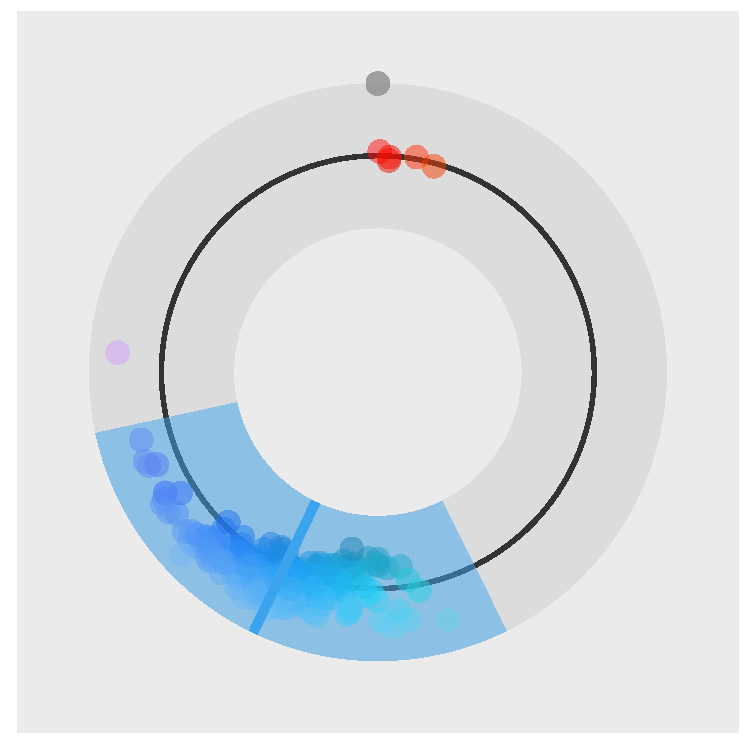
\includegraphics[width=\linewidth]{single_column.pdf}
	\caption{\textbf{A random visualization.} This is an example of a figure that spans only across one of the two columns.}
	\label{fig:column}
\end{figure}

On the other hand, \figurename~\ref{fig:whole} is an example of a figure that spans across the whole page (across both columns) of the report.

% \begin{figure*} makes the figure take up the entire width of the page
\begin{figure*}[ht]\centering 
	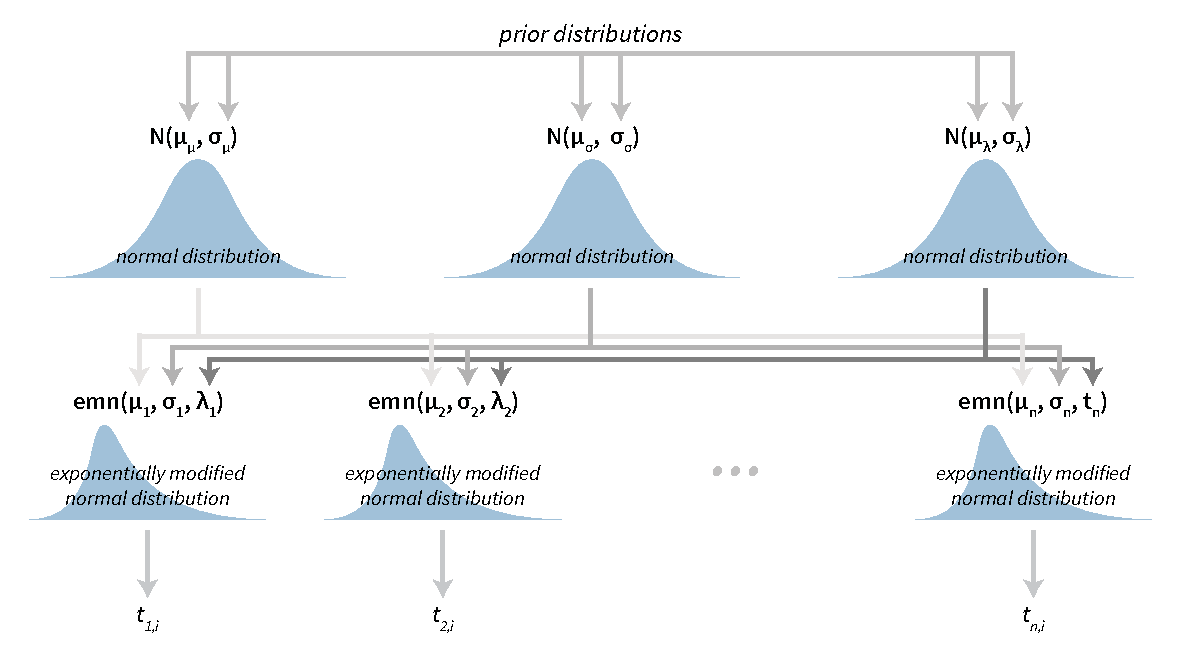
\includegraphics[width=\linewidth]{whole_page.pdf}
	\caption{\textbf{Visualization of a Bayesian hierarchical model.} This is an example of a figure that spans the whole width of the report.}
	\label{fig:whole}
\end{figure*}


\subsection*{Tables}

Use the table environment to insert tables.

\begin{table}[hbt]
	\caption{Table of grades.}
	\centering
	\begin{tabular}{l l | r}
		\toprule
		\multicolumn{2}{c}{Name} \\
		\cmidrule(r){1-2}
		First name & Last Name & Grade \\
		\midrule
		John & Doe & $7.5$ \\
		Jane & Doe & $10$ \\
		Mike & Smith & $8$ \\
		\bottomrule
	\end{tabular}
	\label{tab:label}
\end{table}


\subsection*{Code examples}

You can also insert short code examples. You can specify them manually, or insert a whole file with code. Please avoid inserting long code snippets, advisors will have access to your repositories and can take a look at your code there. If necessary, you can use this technique to insert code (or pseudo code) of short algorithms that are crucial for the understanding of the manuscript.

\lstset{language=Python}
\lstset{caption={Insert code directly from a file.}}
\lstset{label={lst:code_file}}
\lstinputlisting[language=Python]{code/example.py}

\lstset{language=R}
\lstset{caption={Write the code you want to insert.}}
\lstset{label={lst:code_direct}}
\begin{lstlisting}
import(dplyr)
import(ggplot)

ggplot(diamonds,
	   aes(x=carat, y=price, color=cut)) +
  geom_point() +
  geom_smooth()
\end{lstlisting}

%------------------------------------------------

\section*{Results}

Use the results section to present the final results of your work. Present the results in a objective and scientific fashion. Use visualisations to convey your results in a clear and efficient manner. When comparing results between various techniques use appropriate statistical methodology.

\subsection*{More random text}

This text is inserted only to make this template look more like a proper report. Lorem ipsum dolor sit amet, consectetur adipiscing elit. Etiam blandit dictum facilisis. Lorem ipsum dolor sit amet, consectetur adipiscing elit. Interdum et malesuada fames ac ante ipsum primis in faucibus. Etiam convallis tellus velit, quis ornare ipsum aliquam id. Maecenas tempus mauris sit amet libero elementum eleifend. Nulla nunc orci, consectetur non consequat ac, consequat non nisl. Aenean vitae dui nec ex fringilla malesuada. Proin elit libero, faucibus eget neque quis, condimentum laoreet urna. Etiam at nunc quis felis pulvinar dignissim. Phasellus turpis turpis, vestibulum eget imperdiet in, molestie eget neque. Curabitur quis ante sed nunc varius dictum non quis nisl. Donec nec lobortis velit. Ut cursus, libero efficitur dictum imperdiet, odio mi fermentum dui, id vulputate metus velit sit amet risus. Nulla vel volutpat elit. Mauris ex erat, pulvinar ac accumsan sit amet, ultrices sit amet turpis.

Phasellus in ligula nunc. Vivamus sem lorem, malesuada sed pretium quis, varius convallis lectus. Quisque in risus nec lectus lobortis gravida non a sem. Quisque et vestibulum sem, vel mollis dolor. Nullam ante ex, scelerisque ac efficitur vel, rhoncus quis lectus. Pellentesque scelerisque efficitur purus in faucibus. Maecenas vestibulum vulputate nisl sed vestibulum. Nullam varius turpis in hendrerit posuere.

Nulla rhoncus tortor eget ipsum commodo lacinia sit amet eu urna. Cras maximus leo mauris, ac congue eros sollicitudin ac. Integer vel erat varius, scelerisque orci eu, tristique purus. Proin id leo quis ante pharetra suscipit et non magna. Morbi in volutpat erat. Vivamus sit amet libero eu lacus pulvinar pharetra sed at felis. Vivamus non nibh a orci viverra rhoncus sit amet ullamcorper sem. Ut nec tempor dui. Aliquam convallis vitae nisi ac volutpat. Nam accumsan, erat eget faucibus commodo, ligula dui cursus nisi, at laoreet odio augue id eros. Curabitur quis tellus eget nunc ornare auctor.


%------------------------------------------------

\section*{Discussion}

Use the Discussion section to objectively evaluate your work, do not just put praise on everything you did, be critical and exposes flaws and weaknesses of your solution. You can also explain what you would do differently if you would be able to start again and what upgrades could be done on the project in the future.


%------------------------------------------------

\section*{Acknowledgments}

Here you can thank other persons (advisors, colleagues ...) that contributed to the successful completion of your project.

\end{comment}
%----------------------------------------------------------------------------------------
%	REFERENCE LIST
%----------------------------------------------------------------------------------------
\bibliographystyle{unsrt}
\bibliography{report}


\end{document}